\section{}
\[
H(s)=\frac{10\,(1 - s)}{s+10}\,.
\]
\subsection{Bode-Diagramm}
\begin{center}
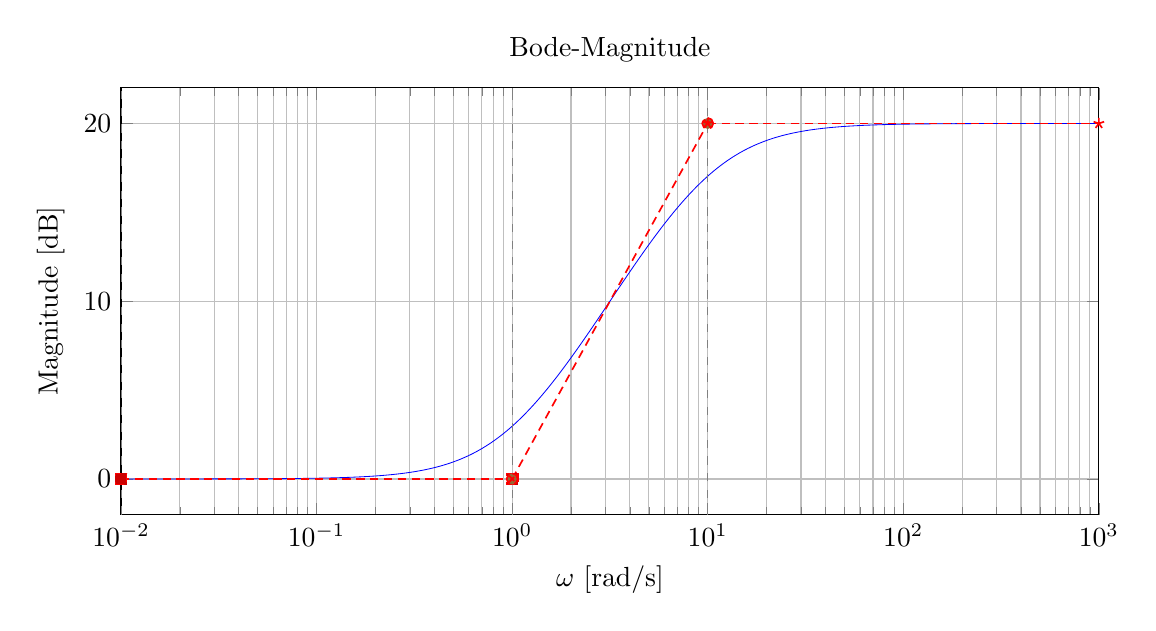
\begin{tikzpicture}
\begin{semilogxaxis}[
  width=14cm,height=7cm,
  xmin=1e-2,xmax=1e3,
  xlabel={$\omega$ [rad/s]},
  ylabel={Magnitude [dB]},
  grid=both,
  ytick distance=10,
  title={Bode-Magnitude}
]
\addplot[
  domain=1e-2:1e3,
  samples=600,
  mark=none,
  ytick distance=10,
  line width=0.3pt,
  blue
] {20 + 20*ln(sqrt(1 + x^2))/ln(10) - 20*ln(sqrt(100 + x^2))/ln(10)};
\addplot+[domain=1e-2:1,samples=2,dashed,dash pattern=on 3pt off 2pt,line width=0.6pt,red] {0};
\addplot+[domain=1:1e1,samples=2,dashed,dash pattern=on 3pt off 2pt,line width=0.6pt,red] {20*ln(x)/ln(10)};
\addplot+[domain=1e1:1e3,samples=2,dashed,dash pattern=on 3pt off 2pt,line width=0.6pt,red] {20};
\draw[gray,dashed] (rel axis cs:0,0) -- (rel axis cs:0,1);
\draw[gray,dashed] (axis cs:1,\pgfkeysvalueof{/pgfplots/ymin}) -- (axis cs:1,\pgfkeysvalueof{/pgfplots/ymax});
\draw[gray,dashed] (axis cs:10,\pgfkeysvalueof{/pgfplots/ymin}) -- (axis cs:10,\pgfkeysvalueof{/pgfplots/ymax});
\node[gray,anchor=south east] at (axis cs:1,\pgfkeysvalueof{/pgfplots/ymax}) {\scriptsize Nullstelle $\omega_z=1$ (RHP)};
\node[gray,anchor=south east] at (axis cs:10,\pgfkeysvalueof{/pgfplots/ymax}) {\scriptsize Pol $\omega_p=10$};
\end{semilogxaxis}
\end{tikzpicture}
\vspace{6mm}
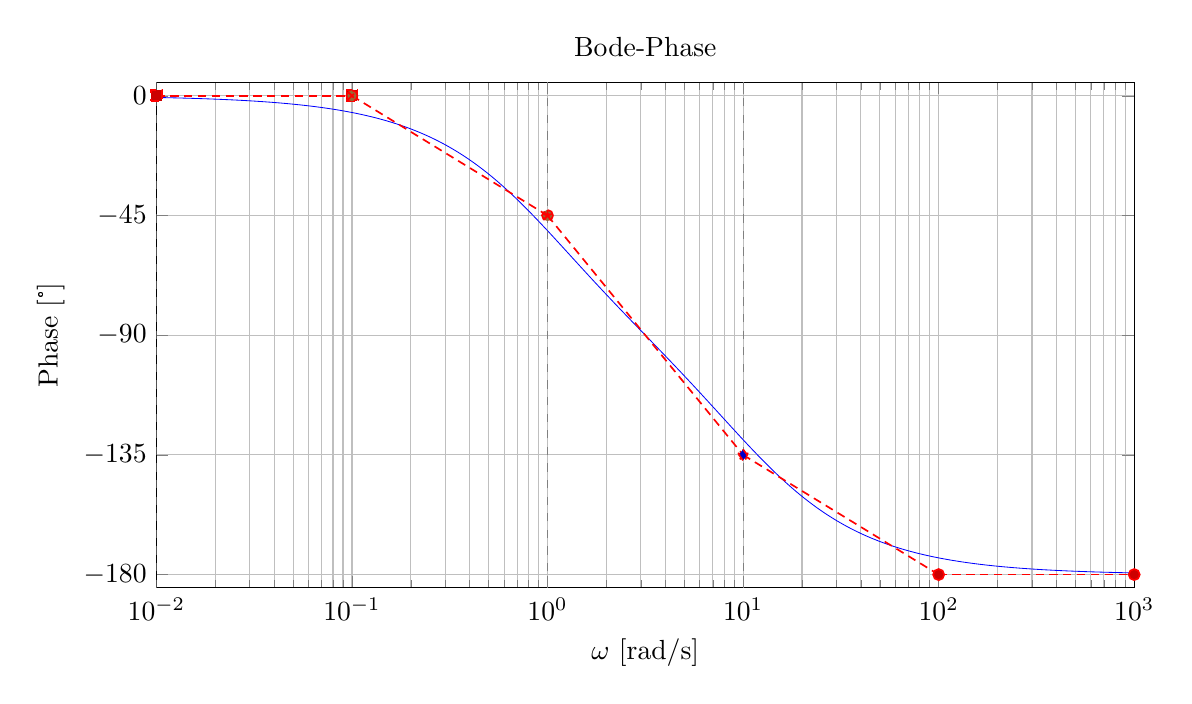
\begin{tikzpicture}
\begin{semilogxaxis}[
  width=14cm,height=8cm,
  xmin=1e-2,xmax=1e3,
  ymin=-185,ymax=5,
  xlabel={$\omega$ [rad/s]},
  ylabel={Phase [°]},
  ytick distance=45,
  grid=both,
  title={Bode-Phase}
]
\addplot[
  domain=1e-2:1e3,
  samples=600,
  mark=none,
  line width=0.3pt,
  blue
] {-atan(x) - atan(x/10)};
\addplot+[domain=1e-2:1e-1,samples=2,dashed,dash pattern=on 3pt off 2pt,line width=0.6pt,red] {0};
\addplot+[domain=1e-1:1e0,samples=2,dashed,dash pattern=on 3pt off 2pt,line width=0.6pt,red] {-45 - 45*ln(x)/ln(10)};
\addplot+[domain=1e0:1e1,samples=2,dashed,dash pattern=on 3pt off 2pt,line width=0.6pt,red]{-45 - 90*ln(x)/ln(10)};
\addplot+[domain=1e1:1e2,samples=2,dashed,dash pattern=on 3pt off 2pt,line width=0.6pt,red] {-135 - 45*ln(x/10)/ln(10)};
\addplot+[domain=1e2:1e3,samples=2,dashed,dash pattern=on 3pt off 2pt,line width=0.6pt,red] {-180};
\draw[gray,dashed] (rel axis cs:0,0) -- (rel axis cs:0,1);
\draw[gray,dashed] (axis cs:1,\pgfkeysvalueof{/pgfplots/ymin}) -- (axis cs:1,\pgfkeysvalueof{/pgfplots/ymax});
\draw[gray,dashed] (axis cs:10,\pgfkeysvalueof{/pgfplots/ymin}) -- (axis cs:10,\pgfkeysvalueof{/pgfplots/ymax});
\node[gray,anchor=south east] at (axis cs:1,\pgfkeysvalueof{/pgfplots/ymax}) {\scriptsize Nullstelle $\omega_z=1$ (RHP)};
\node[gray,anchor=south east] at (axis cs:10,\pgfkeysvalueof{/pgfplots/ymax}) {\scriptsize Pol $\omega_p=10$};
\end{semilogxaxis}
\end{tikzpicture}
\end{center}
\newpage
\subsection{Erklärung}
\begin{description}[leftmargin=1.2em,labelsep=.6em,font=\bfseries]

\item[1. Normalform herstellen.]
Bringe die Übertragungsfunktion exakt in die im Skript definierte Standardform.
\[
H(s)=\frac{10(1-s)}{s+10}
= (1 - sT_z)\cdot\frac{1}{1+sT_p}\,.
\]
mit \(K_0=1\), \(r=0\), \(T_z=1\), \(T_p=\tfrac{1}{10}\).
Klassifiziere die Glieder: RHP-Nullstelle \(\underline{F}_z(s)=(1-sT_z)\) mit \(T_z=1\); reelles Polglied \(\underline{F}_p(s)=\tfrac{1}{1+sT_p}\) mit \(T_p=\tfrac{1}{10}\).


\item[2. Eckfrequenzen bestimmen und sortieren.] Die $\omega$-Eckfrequenzen lassen sich aus den $T_n$'s bestimmen und müssen anschließend sortiert werden:
\[
\omega_z=\frac{1}{T_z}=1\,\mathrm{rad/s},\qquad \omega_p=\frac{1}{T_p}=10\,\mathrm{rad/s},\qquad \omega_z<\omega_p.
\]

\item[3. Startpunkt des Amplitudengangs festlegen (Geradennäherung).]
Wähle \(\omega_{\min}=\omega_z=1\). Regel:
\[
F_{\mathrm{dB}}(\omega_{\min})=20\log_{10}\!\big(|K_0F^*_{ges}(0)|\cdot\omega_{\min}^{\,r}\big)
=20\log_{10}(1)=0\,\mathrm{dB}.
\]
Dieser Punkt ist der Anker der Geradennäherung.

\item[4. Verlauf links vom Startpunkt zeichnen.]
Für \(\omega<\omega_z\) bleibt die Amplituden-Asymptote bei \(0\,\mathrm{dB}\) konstant (Anfangssteigung \(r\cdot 20 \,\mathrm{dB}=0\)). Zeichne eine waagrechte Gerade links von der kleinsten Eckfrequenz.

\item[5. Steigungswechsel an den Eckfrequenzen eintragen.]
Ab der RHP-Nullstelle bei \(\omega_z=1\) nimmt die Steigung um \(+20\,\mathrm{dB/dec}\) zu.
Der Pol bei \(\omega_p=10\) bewirkt einen zusätzlichen Steigungswechsel um \(-20\,\mathrm{dB/dec}\) ab \(\omega=10\).
Netto:
\[
\begin{cases}
0\,\mathrm{dB/dec},& \omega<1,\\
+20\,\mathrm{dB/dec},& 1\le\omega<10,\\
0\,\mathrm{dB/dec},& \omega\ge 10\;\Rightarrow |H|\to 20\,\mathrm{dB}.
\end{cases}
\]
Geradennäherungen:
\[
|H(j\omega)|_{\mathrm{dB}}\approx
\begin{cases}
0,& \omega\le 1,\\
20\log_{10}\omega,& 1<\omega\le 10,\\
20,& \omega\ge 10.
\end{cases}
\]

\item[6. Eckabrundungen korrekt berücksichtigen.]
RHP-Nullstelle: bei \(\omega=\omega_z\) liegt die exakte Magnitude um \(+3\,\mathrm{dB}\) über der Asymptote.
Pol: bei \(\omega=\omega_p\) liegt die exakte Magnitude um \(-3\,\mathrm{dB}\) unter der Asymptote.
Stützpunkte:
\[
|H(j1)|_{\mathrm{dB}}=20+10\log_{10}(2)-10\log_{10}(101)\approx +3\,\mathrm{dB},
\]
\[
|H(j10)|_{\mathrm{dB}}=20+10\log_{10}(101)-10\log_{10}(200)\approx 17\,\mathrm{dB}.
\]

\item[7. Phasenstartwert festlegen.]
Nutze die Regel für \(\omega\to 0\): Da \(K_0F_{ges}(0)>0\) und \(r=0\), ist der Startwert der Phase
\[
\varphi(0)=r \cdot 90^\circ=0^\circ.
\]

\item[8. Phasenänderung durch Nullstelle und Pol eintragen.]
RHP-Nullstelle bei \(\omega_z=1\): Phasenänderung \(-90^\circ\) über die Dekade \([0.1,10]\) (Geradennäherung \(-45^\circ-45^\circ\log_{10}\omega\)).
Pol bei \(\omega_p=10\): zusätzlicher Abfall um \(-90^\circ\) über \([1,100]\) (Geradennäherung \(-45^\circ-45^\circ\log_{10}(\omega/10)\)). Im Intervar $[1,10]$ überlagern sich diese Effekte.
Gesamt:
\[
\varphi(\omega)\approx
\begin{cases}
0^\circ,& \omega\le 0.1,\\
-45^\circ-45^\circ\log_{10}\omega,& 0.1<\omega\le 1,\\
-45^\circ-90^\circ\log_{10}\omega,& 1<\omega\le 10,\\
-135^\circ-45^\circ\log_{10}(\omega/10),& 10<\omega\le 100,\\
-180^\circ,& \omega\ge 100.
\end{cases}
\]

\item[9. Grenzwerte und Konsistenz prüfen.]
DC: \(|H(0)|=1\Rightarrow 0\,\mathrm{dB}\), \(\varphi(0)=0^\circ\).
HF: \(|H(j\omega)|\to 10\Rightarrow 20\,\mathrm{dB}\).
Pol-/Nullzählung bestätigt die Endphase: Zählergrad \(m=-1\), Nennergrad \(n=1\) \(\Rightarrow (m-n)\cdot 90^\circ=0^\circ\); $m=-1$, da die Nullstelle RHP ist.

\end{description}

\subsubsection*{Stückweise Näherungen (für die Skizze)}
\[
|H(j\omega)|_{\mathrm{dB}}\approx
\begin{cases}
0,& \omega\ll 1,\\[2pt]
20\log_{10}\omega,& 1\ll\omega\ll 10,\\[2pt]
20,& \omega\gg 10,
\end{cases}
\]
\[
\varphi(\omega)\approx
\begin{cases}
0^\circ,& \omega\le 0.1,\\[2pt]
-45^\circ-45^\circ\log_{10}\omega,& 0.1<\omega<1,\\[2pt]
-45^\circ-90^\circ\log_{10}\omega,& 1<\omega<10,\\[2pt]
-135^\circ-45^\circ\log_{10}(\omega/10),& 10<\omega<100,\\[2pt]
-180^\circ,& \omega\ge 100.
\end{cases}
\]

\newpage